\chapter{Implementación}

\section{Función de transferencia}

La función de transferencia es la encargada de dar a un valor de intensidad las propiedades de color y opacidad que le corresponden para la visualización del volumen.

En VTK la función de transferencia forma parte de la clase \texttt{vtkVolumeProperty}. Para ello proporciona otras dos clases:
\begin{itemize}
	\item \texttt{vtkColorTransferFunction}: Para definir el color. Se enlaza a \texttt{vtkVolumeProperty} con el método \texttt{SetColor}.
	\item \texttt{vtkPiecewiseFunction}: Para definir el color. Se enlaza a \texttt{vtkVolumeProperty} con el método \texttt{SetScalarOpacity}.
\end{itemize}

Podemos, por tanto, diferenciar dos partes fundamentales en la función de transferencia, la encargada de dar la propiedad de color y la de dar la propiedad de opacidad. Ambas trabajan de forma independiente. Es decir, cuando se define un punto en una de ellas, no tiene por qué definirse en la otra.

\subsection{Color}

Para definir esta función, hay que agregar puntos para valores de intensidad a los que se les asignará un color. VTK se encargará de interpolar entre un punto y otro (Figura \ref{fig:color_tf}). 

Por defecto, cuando no hay ningún punto, a todos los valores de intensidad les corresponderá un color negro. De forma parecida se comporta cuando solo hay un punto pero en lugar de negro, les corresponderá el color del punto que se ha definido.

VTK permite trabajar tanto con HSV como con RGB y para añadir un punto hay que utilizar \texttt{AddHSVPoint} o \texttt{AddRGBPoint}. A estos métodos se les pasa un primer parámetro en coma flotante con el valor de intensidad donde se establecerá ese punto y otros tres con las distintas exponentes (\textit{hue}, \textit{saturation}, \textit{brightness} o \textit{red}, \textit{green}, \textit{blue}).

\begin{figure}[H]
	\centering
	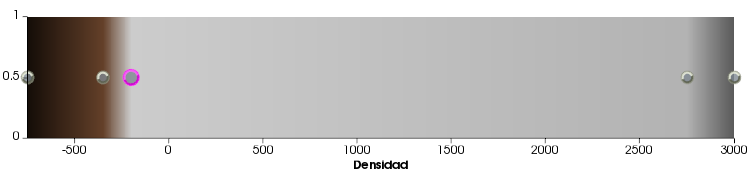
\includegraphics[width=10cm]{imagenes/color_tf}
	\caption{Función de transferencia de color del \textit{preset} \textit{CT-Cardiac} extraído del software Slicer \cite{slicer}}
	\label{fig:color_tf}
\end{figure}

\subsection{Opacidad}

